%
% File: chap01.tex
% Author: Ran Itay
% Description: Introduction chapter.
%
\let\textcircled=\pgftextcircled
\chapter{Introduction}
\label{chap:intro}

\initial{B}egins

%======
\section{Non Linear Emission of Radiation in Liquid Xenon}
\label{sec:intro_superradiance}
As explained in (~\ref{} TODO add reference here) in LXe based experiment the exact properties of the scintillation and ionization responses to all types of interaction must be well quantified and understood. Mainly, much research has been focused on the scintilation and ionization responses of LXe to events with energy recoil as low as <O(10\,keV)~\cite{Manzur:2009hp,Aprile:2012an,Baudis:2013cca}(TODO add LUX).
Specifically the reconstruction of the directionality of recoil nuclei or electrons is of great interest to DM direct detection experiments. Better understanding of these properties may help to reduce background dramatically.

Several existing and proposed experiments such as DRIFT-II~\cite{Muna:2007zz}, DMTPC~\cite{Deaconu:2017vam}, NEWAGE~\cite{Yakabe:2016pjh} and MIMAC~\cite{Riffard:2016mgw}, exploit recoil direction properties. However These experiments are using dilute gas in which the ionization tracks extend to a few millimeters. However, in LXe the track length is estimated to be O(100nm). Moreover the topology of the excimers clouds is represented by a complex structure of branches which are formed by secondary recoils [35,50]. These two different properties, track length and structure, makes it highly difficult if not impossible to construct directionality in a LXe experiment. Therefore, a different approach for directionality measurement needs to be adopted for DM LXe based experiments.

The phenomena of an isolated particle in an excited state undergoing a transition to its ground state (i.e. spontaneous decay) as a result of the vacuum electromagnetic field  is well described in the theory of quantum electrodynamics. This theory is applicable for an ensemble of particles only when particles interact with the vacuum electromagnetic field separately. In this case the ensemble will emit light an exponential law. The characteristic time, $\tau_{sp}$, of a single particle to radiate is equal to the the reciprocal of the transition rate $\Gamma$ from the initially excited level. The radiation pattern in this case is isotropic in its nature, see Fig.~\ref{fig:emissionType}a. 

These radiation properties are significantly different when the radiating particles are dense enough. In this case the collective radiation from  the ensemble is different than the sum of all particles radiating. This phenomena was first postulated by Dicke~\cite{DickeSR} in 1954 and was first measured in Xe by Rosenberger in 1965~\cite{FirstMeasure}. In his research the radiation decay time from a two level atomic system was considered and expected to be dependent on the number of radiating particles N. This type of emission is referred as superradiance. This phenomena is due to interaction of the radiating particles with each other via a common electromagnetic radiation field, which results in a correlation between the atomic dipole moment. This correlation leads to a macroscopic optical polarization proportional to N. Hence the radiation intensity is proportional to $N^2$, leading to a pulsed radiation with duration proportional to $1/N$, see Fig~\ref{fig:emissionType}b. The phenomena of superradiance has been studied extensively since see [TODO add cite [52, 53]]   
\begin{figure}[t!]
	\centering
	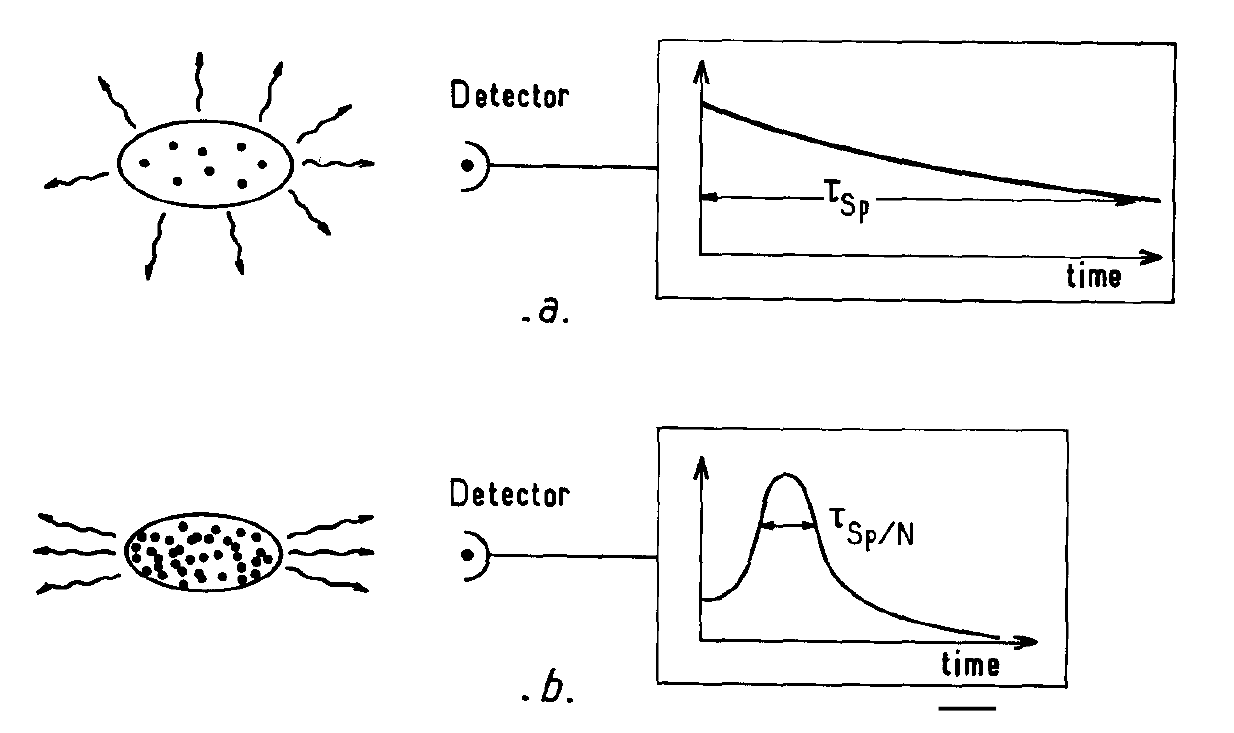
\includegraphics[width=0.8\textwidth]{fig01/emissionTypes.png}
	\mycaption[TODO list of figures caption.]{TODO insert caption here}
	\label{fig:emissionType}
\end{figure}


An effective self-induction of correlations between dipole moments is a necessary condition for a particles to exhibit a \superradiance emission. The condition for this to occur are very different then the ones of regular fluorescence. The characteristic time of \superradiance emission to happen, $\tau_c \sim 1/N $ must be shorter the relaxation time of the atomic dipole moment, $\tau_d$. It also has to be shorter then $\tau_{sp}$, however in most cases, $\tau_{d}$ is smaller than $\tau_{sp}$, hence this is a more stiringit condition. Notice that unlike inverse population that happens in lasers, which occurs due to an external "pump", the correlation build-up between the radiating particles in \superradiance happens spontaneously in the course of emission process.

The geometry of the radiating particle ensemble influences greatly weather or not a system will exhibit a \superradiance or standard spontaneous emissions. Specifically the two relevant quantities, are the wavelength $\lambda$ of the emitted photon, and the size of the radiating particles cloud. A system with linear size much smaller then the emitted photons wavelength.   
%The superradiant emission depends strongly on the geometry of the atomic system. The length
%scale relevant for the qualitative behaviour of the emitted radiation is the wavelength , λ, corresponding
%to the atomic de-excitation. If we consider a system of radiators with linear size much
%smaller than λ, i.e. V  λ
%3
%, where V is the volume of the system, the system will emit a pulse in an
%arbitrary direction (isotropic), with an intensity that will reach a maximum Imax ∼ N2
%. However,
%a system with linear size L & λ will radiate most of its energy into small solid angles along the

TODO understand previous paragraph

\section{EFT}
\label{sec:intro_EFT}

The traditional approach for computing predictions of the rate of WIMP-nucleon scattering has been to take only leading-order terms in a WIMP-nucleon effective field theory (EFT) with a very simple treatment of nuclear structure~\cite{LEWIN}. This leads to two main types of interactions, which are commonly labelled ``Spin Independent'' (SI) and ``Spin Dependent'' (SD). However, in recent years many authors have pointed out that in certain theories these interactions may be suppressed or nonexistent, such that otherwise subleading interactions may dominate the scattering process~\cite{Chang:2009yt}. To account for this possibility in a systematic way, a more sophisticated EFT approach has been developed ~\cite{Fitzpatrick:2012ib,Anand:MathTools,Fitzpatrick:MathTools}. In the new approach, an effective Lagrangian describing the WIMP-nucleus interaction is constructed, that takes into account all Galilean-invariant operators up to second order in the momentum exchange. This framework introduces new operators associated with different types of nuclear responses, along with the standard SI and SD ones, resulting in a set of fourteen operators $\mathcal{O}_i$ which may couple independently to protons and neutrons. In Eqs. (\ref{eq:OpDef}) we list these operators following the convention from~\cite{Anand:MathTools}. The operators depend explicitly on 4 linearly independent quantities: $\vec{v}^{\perp} \equiv \vec{v} + \frac{\vec{q}}{2\mu_N} $, the relative perpendicular velocity between the WIMP and the nucleon, $\vec{q}$, the momentum transferred in the scattering event, and $\vec{S}_\chi$, $\vec{S}_N$, the WIMP and nucleon spins. $\mathcal{O}_2$ is not considered here as it cannot be obtained from a relativistic operator at leading order.
%

\begingroup
\belowdisplayskip=0pt
\begin{align*}
\begin{split} 
&\mathcal{O}_1 = 1_{\chi} 1_N  \\
%&\mathcal{O}_2 = (v^{\perp})^2 \\
&\mathcal{O}_3 = i\vec{S}_N\cdot (\frac{\vec{q}}{m_N}\times\vec{v}^\perp) \\
&\mathcal{O}_4 = \vec{S}_{\chi}\cdot \vec{S}_N \\
&\mathcal{O}_5 = i\vec{S}_{\chi}\cdot (\frac{\vec{q}}{m_N}\times\vec{v}^\perp) \\
&\mathcal{O}_6 = (\vec{S}_{\chi} \cdot \frac{\vec{q}}{m_N})(\vec{S}_N \cdot \frac{\vec{q}}{m_N}) \\
&\mathcal{O}_7 = \vec{S}_N \cdot \vec{v}^\perp \\
&\mathcal{O}_8 = \vec{S}_{\chi} \cdot \vec{v}^\perp  \\
\end{split}
\begin{split}
&\mathcal{O}_9 = i\vec{S}_{\chi} \cdot(\vec{S}_N \times \frac{\vec{q}}{m_N}) \\
&\mathcal{O}_{10} = i\vec{S}_N \cdot (\frac{\vec{q}}{m_N}) \\
&\mathcal{O}_{11} = i\vec{S}_{\chi} \cdot (\frac{\vec{q}}{m_N}) \\
&\mathcal{O}_{12} = \vec{S}_\chi \cdot (\vec{S}_N \times \vec{v}^\perp) \\
&\mathcal{O}_{13} = i(\vec{S}\chi \cdot \vec{v}^\perp)(\vec{S}_N \cdot \frac{\vec{q}}{m_N})\\
&\mathcal{O}_{14} = i(\vec{S}_\chi \cdot \frac{\vec{q}}{m_N})(\vec{S}_N \cdot \vec{v}^\perp) \\
\end{split}
\end{align*}
\endgroup
\begingroup
\abovedisplayskip=0pt
\begin{align}
&\mathcal{O}_{15} = -(\vec{S}_\chi \cdot \frac{\vec{q}}{m_N})\left[(\vec{S}_N \times \vec{v}^\perp)\cdot \frac{\vec{q}}{m_N}\right]
\label{eq:OpDef}
\end{align}
\endgroup

Unlike the more commonly studied types of interaction (SI,SD), which are not suppressed when $\vec{q} \rightarrow 0$ and for which the scattering rate on nucleons is expected to be largest for low energy nuclear recoils, some of the new EFT operators depend explicitly on $\vec{q}$ and so their interaction cross section is suppressed for low momentum transfers. Consequently, their scattering rate peaks at non-zero nuclear recoil energy. For sufficiently high WIMP masses, this may even occur outside typical analysis windows, which usually have an upper range of around $ 43\,\keVr$ (nuclear recoil equivalent
energy) since they are designed to search for SI and SD interactions, which predict exponentially-falling recoil spectra (see Figure~\ref{fig:dRdE}). Due to the theoretical bias of only considering SI and SD interactions, high energy nuclear recoils remain unexplored in many experiments.

	    Another typical assumption that can be relaxed is that WIMPs should scatter elastically with nuclei. There exist dark matter models in which the incoming and outgoing WIMPs have different mass states~\cite{InelasticIntro} separated by a keV-scale splitting. In the case where the outgoing state is more massive than the incoming state, the cross section for low recoil energies can again be suppressed, this time by scattering kinematics. Recently an inelastic adaptation of the EFT operator framework discussed above was developed~\cite{InelasticMath}. In this case the operators presented in Eqs.~\ref{eq:OpDef} are modified such that $\vec{v}^\perp_{inelastic} = \vec{v}^\perp_{elastic} +\frac{\delta_m}{\vert{\vec{q}}\vert^2}\vec{q}$. We consider this case in section \ref{subsubsec:Inelastic}.
%\subsection{Subsection}
%\label{subsec:subsec01}
%
%Begins a subsection.
%
%%A figures matrix.
%\begin{figure}[t!]
%\centering
%\begin{minipage}{3.3cm}
%    \centering
%    \subtop[]{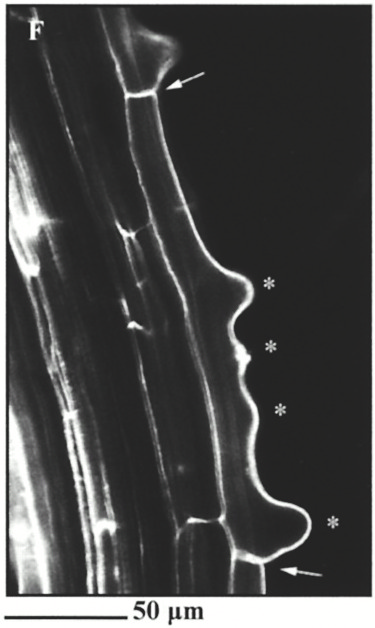
\includegraphics[height=0.28\textheight]{fig01/Nswellings}\label{sf:multiRH02a}}
%\end{minipage}
%\hspace{0.5cm}
%\begin{minipage}{3.3cm}
%    \centering
%    \subtop[]{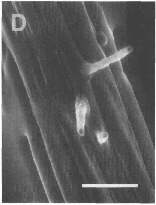
\includegraphics[height=0.27\textheight]{fig01/Mswellings}\label{sf:multiRH02b}}
%\end{minipage}
%\hspace{1.3cm}
%\begin{minipage}{3.3cm}
%    \centering
%    \subtop[]{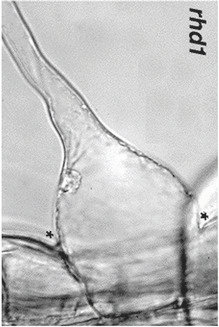
\includegraphics[height=0.27\textheight]{fig01/rhd1}\label{sf:multiRH02c}}
%\end{minipage}
%\\ \vspace{0.1cm}
%\begin{minipage}{10cm}
%    \centering
%    \subtop[]{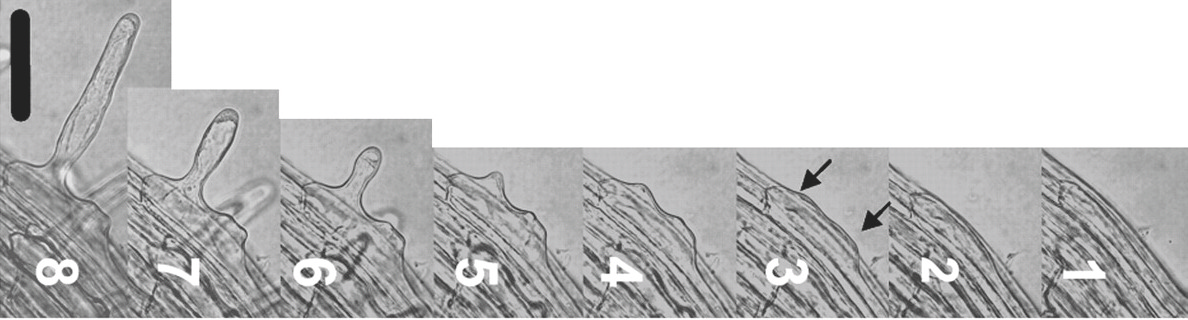
\includegraphics[height=0.145\textheight]{fig01/mutantrhd6}\label{sf:multiRH02d}}
%\end{minipage}
%\\ \vspace{0.1cm}
%\begin{minipage}{10cm}
%    \centering
%    \subtop[]{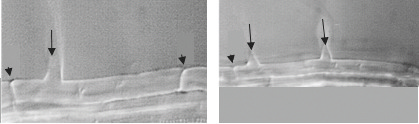
\includegraphics[height=0.16\textheight]{fig01/auxab}\label{sf:multiRH02e}}
%\end{minipage}
%\mycaption[Hair-forming mutant cells.]{(a) A mutant RH cell. Asterisks show multiple sites of RH initiation in a single root hair cell (indicated by the arrows). Figure reproduced from \cite{rigas01}. (b)~Hair-forming cell with three RH initiation locations. The bar represents $50\mu m$. Figure reproduced from \cite{massuci01}. (c) Large bump in mutant {\itshape rhd1}. Figure reproduced from \cite{griersonRH}. (d) Mutant overexpressing gene {\itshape ROP2}; from right-hand to left-hand, numbers indicate progressive snapshots at different times. RH initiation sites are indicated by the arrows. The bar represents $75\mu m$. Figure reproduced from~\cite{mjones01}. (e)~Mutants affected by auxin. On the left-hand side, RH site is farther away from the apical end (left arrow cap); on the right-hand side, multiple RH locations (arrows). Figure reproduced from~\cite{payne01}.}
%\label{fig:multiRH02}
%\end{figure}
%
%% A single figure
%\begin{figure}[t!]
%	\centering
%	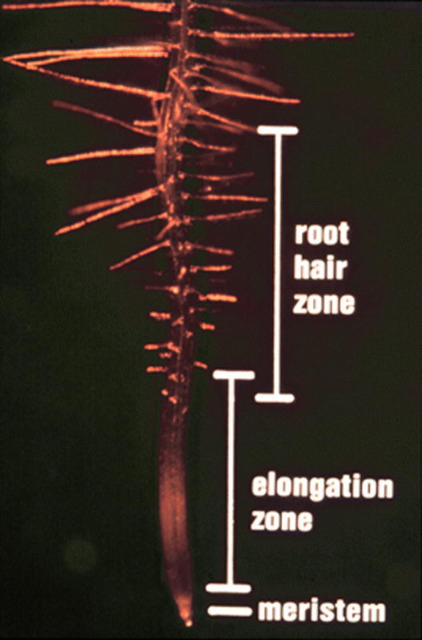
\includegraphics[height=0.35\textheight]{fig01/devepzones}
%	\mycaption[Developmental zones of an Arabidopsis root.]{Developmental zones of an Arabidopsis root. Figure reproduced from \cite{griersonRH}.}
%	\label{fig:RHP02}
%\end{figure}

%=========================================================